%!TEX root = vaisagh_thesis.tex
\chapter{Conclusion and Future Work}
\label{chapter:finale}

The previous chapters have introduced the IBEVAC architectures and it's constituent models. Only the IBP module has been implemented so far. The preliminary design of the remaining modules was discussed in Chapter~\ref{chapter:TheRemainingModules}. However, design work still needs to be done before the model design can be finalized. In Sect.~\ref{CFW:ModelDesign}, an expected time frame for finalizing the design details of the model is first discussed. Following this, in Sect.~\ref{CFW:Implementation}, some of the implementation details and tools used are discussed along with an estimated schedule for completion of implementation of the model. Finally, some of the work involved in validation of the model is then presented in Sect.~\ref{CFW:Validation}. However, before the future work and plan of action is discussed, Sect.~\ref{CFW:Conclusion} first summarizes and concludes the report.


\section{Summary and Conclusion}
\label{CFW:Conclusion}

In the beginning of this report, the idea of crowd egress simulation and the importance of modeling accurately the entire process of evacuation right from the pre-evacuation behavior to the time where all the evacuees have evacuated the building was introduced. Then a brief overview of the limitations of existing models. The information based approach to modeling crowd egress that is presented in this report was intorduced next.

Chapter~\ref{chapter:LiteratureReview} gave a comprehensive overview of the literature. The multidisciplinary nature of the problem was presented next; this was followed by a detailed discussion of the current state of our knowledge of human behavior process in fire evacuations. The various crowd behavior theories developed over the years was introduced and an analysis of the similarities and differences of these models was presented. This was followed by an overview of the different approaches to the problem of computationally modeling and studying a crowd evacuation. This was followed by a detailed analysis of some notable models and the strengths and weaknesses of these models.

Chapter~\ref{chapter:IBEVAC} introduced a complete information based model of an agent complete with an information based perception system, a communication engine, a memory system, a decision making engine and a navigation system.

A basic Information Based Perception~(IBP) model has already been developed and it was presented in Chapter~\ref{chapter:IBP}. The chapter also presented some simulation results that illustrated the effects of using an Information Based Perception on motion planning. In Chapter~\ref{chapter:TheRemainingModules}, the other modules in the model were presented along with some of the related work and basic details of each module.

Finally, this chapter presented a breakdown of the future work that remains along with an estimated time frame for completion of each of these tasks. These are illustrated in Fig.~\ref{fig:GanttChart}.


\section{Future Work}
\label{CFW:FutureWork}
This section discusses the work that remains to be done for the completion of this thesis. As mentioned above, this section is subdivided into three sections highlighting the work remaining in model design, implementation and validation. A Gantt chart figuratively illustrating the schedule proposed in this section is shown in Fig.~\ref{fig:GanttChart} at the end of this chapter.


\section{Tools Used}
\label{CFW:Implementation}

The \emph{implementation} of a model refers to the process of converting the conceptual design into code, i.e.\ a computational model. The section presents some of the details of the implementation like the tools used and the existing work on which the model is built. Section~\ref{CFW:TimeFrame} then presents an estimated time-frame for completion of different implementation related tasks.


\subsubsection{The MASON framework}
\label{CFW:MASON}
The IBEVAC model is implemented in Java using the MASON framework~\cite{Luke:2005wc}. MASON consists of a discrete event simulation core and visualization library that can be used for agent based simulations with a large number of agents. The framework provides features to allow modelers to run multiple replications and create checkpoints from which simulations can be restarted easily. The ease of implementation of inspectors to study particular agents or other aspects of the model and integration with java media framework library (for videos and snapshots), jGraph and java3D make MASON especially appealing for the purpose of this simulation. The framework internally adopts the model-view-controller pattern and completely decouples the view from the controller and the model and makes it easy for a modeler to adopt the same approach. This is critical for studying simulations because a visualization need only be used when particular parts of the simulation need to be observed and analyzed and at all other times more simulations can be run without the additional computational burden of visualization.



\subsubsection{DEPATHSS}
\label{CFW:Depathss}

DEPATHSS is a simulation system for symbiotic simulations of evacuation scenarios (Screenshot in Fig.~\ref{fig:DEPATHSSScreenShot}). It is not directly related to the IBEVAC model. However, the Java based implementation of the simulation system provided a good starting point for implementation of the IBEVAC model and helps remove a lot of programming work that might have been required if the model had to be implemented from scratch.

A Finite Difference Model based implementation of fire propagation used in DEPATHSS is adapted to the MASON framework to simulate fire and smoke propagation in IBEVAC. The smoke will be given a higher diffusion rate so that it spreads at a faster rate.

\begin{figure}[!tb]
\centering
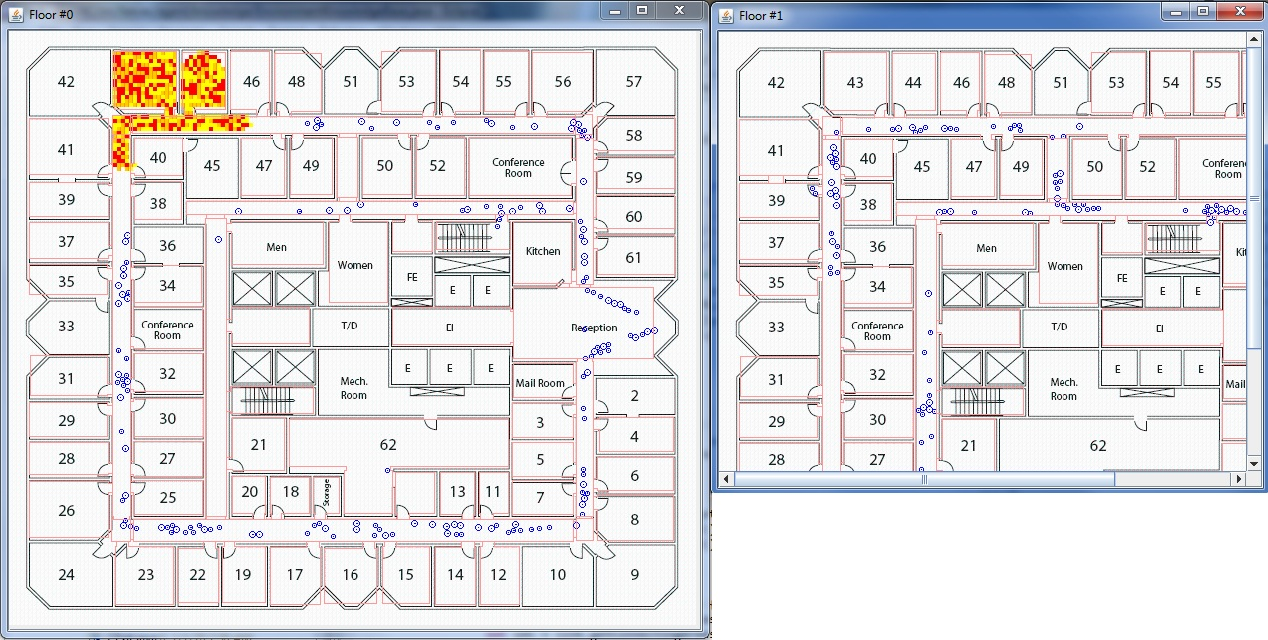
\includegraphics[width=\textwidth]{HiekoSimulationMultiFloor}
\caption[DEPATHSS Screenshot]{This figure shows a screenshot of the evacuation simulation using DEPATHSS of a 2-floor office building with fire propogation modelled (The red, yellow and orange color at the top left of the screen on the first floor). Agents are in blue.}
\label{fig:DEPATHSSScreenShot}
\end{figure}

Another very useful feature of the DEPATHSS system is the ability to create and store layouts of buildings in a generic XML format that can be easily imported into the model. This will be invaluable during experimentation and validation.

As mentioned earlier, the DEPATHSS system's navigation system is being extended to use the 4-level navigation architecture mentioned in this paper. This navigation system can also be integrated into the IBEVAC architecture without much difficulty.

Like the navigation system DEPATHSS is also currently being extended with simple personal cognitive maps for agents and knowledge transfer between agents. This can initially be used in IBEVAC while developing the other modules. Once the other modules have been developed the Communication and Environment Knowledge Modules can be modeled as required by replacing the existing system.

All this implies that, most of the lower level tasks like the framework, basic goal directed navigation and fire and smoke simulation have been completed and tested and most of the work remains only in implementing a higher level behavioral model which is the key contribution of this thesis. An estimate of the time frame required for different aspects of this implementation is considered next.



